\chapter{Latent linear models}


\section{Factor analysis}
One problem with mixture models is that they only use a single latent variable to generate the observations. In particular, each observation can only come from one of $K$ prototypes. One can think of a mixture model as using $K$ hidden binary variables, representing a one-hot encoding of the cluster identity. But because these variables are mutually exclusive, the model is still limited in its representational power.

An alternative is to use a vector of real-valued latent variables,$\vec{z}_i \in \mathbb{R}^L$. The simplest prior to use is a Gaussian (we will consider other choices later):
\begin{equation}\label{eqn:FA-prior}
p(\vec{z}_i)=\mathcal{N}(\vec{z}_i|\vec{\mu}_0,\vec{\Sigma}_0)
\end{equation}
If the observations are also continuous, so $\vec{x}_i \in \mathbb{R}^D$, we may use a Gaussian for the likelihood. Just as in linear regression, we will assume the mean is a linear function of the (hidden) inputs, thus yielding
\begin{equation}\label{eqn:FA-class-conditional-density}
p(\vec{x}_i|\vec{z}_i,\vec{\theta})=\mathcal{N}(\vec{x}_i|\vec{W}\vec{z}_i+\vec{\mu},\vec{\Psi})
\end{equation}
where \vec{W} is a $D \times L$ matrix, known as the \textbf{factor loading matrix}, and $\vec{\Psi}$ is a $D \times D$ covariance matrix. We take $\vec{\Psi}$ to be diagonal, since the whole point of the model is to “force” $\vec{z}_i$ to explain the correlation, rather than “baking it in” to the observation’s covariance. This overall model is called \textbf{factor analysis} or \textbf{FA}. The special case in which $\vec{\Psi}=\sigma^2\vec{I}$ is called \textbf{probabilistic principal components analysis} or \textbf{PPCA}. The reason for this name will become apparent later.


\subsection{FA is a low rank parameterization of an MVN}
FA can be thought of as a way of specifying a joint density model on $\vec{x}$ using a small number of parameters. To see this, note that from Equation \ref{eqn:Linear-Gaussian-system-normalizer}, the induced marginal distribution $p(\vec{x}_i|\vec{\theta})$ is a Gaussian:
\begin{align}
p(\vec{x}_i|\vec{\theta}) & = \int \mathcal{N}(\vec{x}_i|\vec{W}\vec{z}_i+\vec{\mu},\vec{\Psi})\mathcal{N}(\vec{z}_i|\vec{\mu}_0,\vec{\Sigma}_0)\mathrm{d}\vec{z}_i \nonumber \\
 & = \mathcal{N}(\vec{x}_i|\vec{W}\vec{\mu}_0+\vec{\mu},\vec{\Psi}+\vec{W}\vec{\Sigma}_0\vec{W})
\end{align}
From this, we see that we can set $\vec{\mu}_0=0$ without loss of generality, since we can always absorb $\vec{W}\vec{\mu}_0$ into $\vec{\mu}$. Similarly, we can set $\vec{\Sigma}_0=\vec{I}$ without loss of generality, because we can always “emulate” a correlated prior by using defining a new weight matrix, $\tilde{\vec{W}}=\vec{W}\vec{\Sigma}_0^{-\frac{1}{2}}$. So we can rewrite Equation \ref{eqn:FA-prior} and \ref{eqn:FA-class-conditional-density} as:
\begin{align}
p(\vec{z}_i)&=\mathcal{N}(\vec{z}_i|\vec{0},\vec{I}) \\
p(\vec{x}_i|\vec{z}_i,\vec{\theta})&=\mathcal{N}(\vec{x}_i|\vec{W}\vec{z}_i+\vec{\mu},\vec{\Psi})
\end{align}

We thus see that FA approximates the covariance matrix of the visible vector using a low-rank decomposition:
\begin{equation}\label{eqn:FA-prior}
\vec{C} \triangleq \mathrm{cov}[\vec{x}]=\vec{W}\vec{W}^T+\vec{\Psi}
\end{equation}
This only uses $O(LD)$ parameters, which allows a flexible compromise between a full covariance Gaussian, with $O(D^2)$ parameters, and a diagonal covariance, with $O(D)$ parameters. Note that if we did not restrict $\vec{\Psi}$ to be diagonal, we could trivially set $\vec{\Psi}$ to a full covariance matrix; then we could set $\vec{W}=0$, in which case the latent factors would not be required.


\subsection{Inference of the latent factors}
\begin{align}
p(\vec{z}_i|\vec{x}_i,\vec{\theta}) & = \mathcal{N}(\vec{z}_i|\vec{\mu}_i,\vec{\Sigma}_i) \\
\vec{\Sigma}_i & \triangleq (\vec{\Sigma}_0^{-1}+\vec{W}^T\vec{\Psi}^{-1}\vec{W})^{-1} \\
               & =(\vec{I}+\vec{W}^T\vec{\Psi}^{-1}\vec{W})^{-1} \\
\vec{\mu}_i & \triangleq \vec{\Sigma}_i[\vec{W}^T\vec{\Psi}^{-1}(\vec{x}_i-\vec{\mu})+\vec{\Sigma}_0^{-1}\vec{\mu}_0] \\
            & =\vec{\Sigma}_i\vec{W}^T\vec{\Psi}^{-1}(\vec{x}_i-\vec{\mu})
\end{align}
Note that in the FA model, $\vec{\Sigma}_i$ is actually independent of $i$, so we can denote it by $\vec{\Sigma}$. Computing this matrix takes $O(L^3+L^2D)$ time, and computing each $\vec{\mu}_i=\mathbb{E}[\vec{z}_i|\vec{x}_i,\vec{\theta}]$ takes $O(L^2+LD)$ time. The $\vec{\mu}_i$ are sometimes called the \textbf{latent scores}, or \textbf{latent factors}.


\subsection{Unidentifiability}
Just like with mixture models, FA is also unidentifiable. To see this, suppose $\vec{R}$ is an arbitrary orthogonal rotation matrix, satisfying $\vec{R}\vec{R}^T=\vec{I}$. Let us define $\tilde{\vec{W}}=\vec{W}\vec{R}$, then the likelihood function of this modified matrix is the same as for the unmodified matrix, since $\vec{W}\vec{R}\vec{R}^T\vec{W}^T+\vec{\Psi}=\vec{W}\vec{W}^T+\vec{\Psi}$. Geometrically, multiplying $\vec{W}$ by an orthogonal matrix is like rotating $\vec{z}$ before generating $\vec{x}$.

To ensure a unique solution, we need to remove $L(L-1)/2$ degrees of freedom, since that is the number of orthonormal matrices of size $L \times L$.\footnote{To see this, note that there are $L-1$ free parameters in $\vec{R}$ in the first column (since the column vector must be normalized to unit length), there are $L-2$ free parameters in the second column (which must be orthogonal to the first), and so on.} In total, the FA model has $D+LD-L(L-1)/2$ free parameters (excluding the mean), where the first term arises from $\vec{\Psi}$. Obviously we require this to be less than or equal to $D(D+1)/2$, which is the number of parameters in an unconstrained (but symmetric) covariance matrix. This gives us an upper bound on $L$, as follows:
\begin{equation}
L_{\mathrm{max}}=\lfloor D+0.5(1-\sqrt{1+8D}) \rfloor
\end{equation}

For example, $D=6$ implies $L \leq 3$. But we usually never choose this upper bound, since it would result in overfitting (see discussion in Section \ref{sec:FA-Choosing-L} on how to choose $L$).


Unfortunately, even if we set $L < L_{\mathrm{max}}$, we still cannot uniquely identify the parameters, since the rotational ambiguity still exists. Non-identifiability does not affect the predictive performance of the model. However, it does affect the loading matrix, and hence the interpretation of the latent factors. Since factor analysis is often used to uncover structure in the data, this problem needs to be addressed. Here are some commonly used solutions:
\begin{itemize}
\item{\textbf{Forcing $\vec{W}$ to be orthonormal} Perhaps the cleanest solution to the identifiability problem is to force $\vec{W}$ to be orthonormal, and to order the columns by decreasing variance of the corresponding latent factors. This is the approach adopted by PCA, which we will discuss in Section \ref{sec:PCA}. The result is not necessarily more interpretable, but at least it is unique.}
\item{\textbf{Forcing $\vec{W}$ to be lower triangular} One way to achieve identifiability, which is popular in the Bayesian community (e.g., (Lopes and West 2004)), is to ensure that the first visible feature is only generated by the first latent factor, the second visible feature is only generated by the first two latent factors, and so on. For example, if $L=3$ and $D=4$, the correspond factor loading matrix is given by
\begin{equation*}
\vec{W}=\left(\begin{array}{ccc}
w_{11} & 0 & 0 \\
w_{21} & w_{22} & 0 \\
w_{31} & w_{32} & w_{33} \\
w_{41} & w_{32} & w_{43}
\end{array}\right)
\end{equation*}
We also require that $w_{jj} >0$ for $j =1:L$. The total number of parameters in this constrained matrix is $D+DL-L(L-1)/2$, which is equal to the number of uniquely identifiable parameters. The disadvantage of this method is that the first $L$ visible variables, known as the \textbf{founder variables}, affect the interpretation of the latent factors, and so must be chosen carefully.}
\item{\textbf{Sparsity promoting priors on the weights} Instead of pre-specifying which entries in $\vec{W}$ are zero, we can encourage the entries to be zero, using $\ell_1$ regularization (Zou et al. 2006), ARD (Bishop 1999; Archambeau and Bach 2008), or spike-and-slab priors (Rattray et al. 2009). This is called sparse factor analysis. This does not necessarily ensure a unique MAP estimate, but it does encourage interpretable solutions. See Section 13.8 TODO.}
\item{\textbf{Choosing an informative rotation matrix} There are a variety of heuristic methods that try to find rotation matrices $\vec{R}$ which can be used to modify $\vec{W}$(and hence the latent factors) so as to try to increase the interpretability, typically by encouraging them to be (approximately) sparse. One popular method is known as \textbf{varimax}(Kaiser 1958).}
\item{\textbf{Use of non-Gaussian priors for the latent factors} In Section \ref{sec:ICA}, we will dicuss how replacing $p(\vec{z}_i)$ with a non-Gaussian distribution can enable us to sometimes uniquely identify $\vec{W}$ as well as the latent factors. This technique is known as ICA.}
\end{itemize}


\subsection{Mixtures of factor analysers}
The FA model assumes that the data lives on a low dimensional linear manifold. In reality, most
data is better modeled by some form of low dimensional \emph{curved} manifold. We can approximate a curved manifold by a piecewise linear manifold. This suggests the following model: let the $k$'th linear subspace of dimensionality $L_k$ be represented by $\vec{W}_k$, for $k=1:K$. Suppose we have a latent indicator $qi \in \{1,\cdots,K\}$ specifying which subspace we should use to generate the data. We then sample $\vec{z}_i$ from a Gaussian prior and pass it through the $\vec{W}_k$ matrix (where $k=q_i$), and add noise. More precisely, the model is as follows:
\begin{align}
p(q_i|\vec{\theta}) & =\mathrm{Cat}(q_i\vec{\pi}) \\
p(\vec{z}_i|\vec{\theta}) & =\mathcal{N}(\vec{z}_i|\vec{0},\vec{I}) \\
p(\vec{x}_i|q_i=k,\vec{z}_i,\vec{\theta}) & =\mathcal{N}(\vec{x}_i|\vec{W}\vec{z}_i+\vec{\mu}_k,\vec{\Psi})
\end{align}
This is called a \textbf{mixture of factor analysers}(MFA) (Hinton et al. 1997).

Another way to think about this model is as a low-rank version of a mixture of Gaussians. In particular, this model needs $O(KLD)$ parameters instead of the $O(KD^2)$ parameters needed for a mixture of full covariance Gaussians. This can reduce overfitting. In fact, MFA is a good generic density model for high-dimensional real-valued data.


\subsection{EM for factor analysis models}
Below we state the results without proof. The derivation can be found in (Ghahramani and Hinton 1996a). To obtain the results for a single factor analyser, just set $r_{ic} =1$ and $c=1$ in the equations below. In Section \ref{sec:EM-for-PCA} we will see a further simplification of these equations that arises when fitting a PPCA model, where the results will turn out to have a particularly simple and elegant interpretation.

In the E-step, we compute the posterior responsibility of cluster $k$ for data point $i$ using
\begin{equation}
r_{ik} \triangleq p(q_i=k|\vec{x}_i,\vec{\theta}) \propto \pi_k\mathcal{N}(\vec{x}_i|\vec{\mu}_k,\vec{W}_k\vec{W}_k^T\vec{\Psi}_k)
\end{equation}

The conditional posterior for $\vec{z}_i$ is given by
\begin{align}
p(\vec{z}_i|\vec{x}_i,q_i=k,\vec{\theta}) & = \mathcal{N}(\vec{z}_i|\vec{\mu}_{ik},\vec{\Sigma}_{ik}) \\
\vec{\Sigma}_{ik} & \triangleq (\vec{I}+\vec{W}_k^T\vec{\Psi}_k^{-1}\vec{W})_k^{-1} \\
\vec{\mu}_{ik} & \triangleq \vec{\Sigma}_{ik}\vec{W}_k^T\vec{\Psi}_k^{-1}(\vec{x}_i-\vec{\mu}_k)
\end{align}

In the M step, it is easiest to estimate $\vec{\mu}_k$ and $\vec{W}_k$ at the same time, by defining $\tilde{\vec{W}}_k=(\vec{W}_k,\vec{\mu}_k)$, $\tilde{\vec{z}}=(\vec{z},1)$, also, define
\begin{align}
\tilde{\vec{W}}_k & =(\vec{W}_k,\vec{\mu}_k) \\
\tilde{\vec{z}} & =(\vec{z},1) \\
\vec{b}_{ik} & \triangleq \mathbb{E}[\tilde{\vec{z}}|\vec{x}_i,q_i=k]=\mathbb{E}[(\vec{\mu}_{ik};1)] \\
\vec{C}_{ik} & \triangleq \mathbb{E}[\tilde{\vec{z}}\tilde{\vec{z}}^T|\vec{x}_i,q_i=k] \\
    & =\left(\begin{array}{cc}
\mathbb{E}[\vec{z}\vec{z}^T|\vec{x}_i,q_i=k] & \mathbb{E}[\vec{z}|\vec{x}_i,q_i=k] \\
\mathbb{E}[\vec{z}|\vec{x}_i,q_i=k]^T & 1
\end{array}\right)
\end{align}
Then the M step is as follows:
\begin{align}
\hat{\pi}_k & = \frac{1}{N}\sum\limits_{i=1}^N r_{ik} \\
\hat{\tilde{\vec{W}}}_k & = \left(\sum\limits_{i=1}^N r_{ik}\vec{x}_i\vec{b}_{ik}^T\right)\left(\sum\limits_{i=1}^N r_{ik}\vec{x}_i\vec{C}_{ik}^T\right)^{-1} \label{eqn:FA-EM-W} \\
\hat{\vec{\Psi}} & = \frac{1}{N}\mathrm{diag}\left[\sum\limits_{i=1}^N r_{ik}(\vec{x}_i-\hat{\tilde{\vec{W}}}_{ik}\vec{b}_{ik})\vec{x}_i^T\right]
\end{align}

Note that these updates are for “vanilla” EM. A much faster version of this algorithm, based on ECM, is described in (Zhao and Yu 2008).


\subsection{Fitting FA models with missing data}
\label{sec:Fitting-FA-models-with-missing-data}
In many applications, such as collaborative filtering, we have missing data. One virtue of the EM approach to fitting an FA/PPCA model is that it is easy to extend to this case. However, overfitting can be a problem if there is a lot of missing data. Consequently it is important to perform MAP estimation or to use Bayesian inference. See e.g., (Ilin and Raiko 2010) for details.


\section{Principal components analysis (PCA)}
\label{sec:PCA}
Consider the FA model where we constrain $\vec{\Psi}=\sigma^2\vec{I}$, and $\vec{W}$ to be orthonormal. It can be shown (Tipping and Bishop 1999) that, as $\sigma^2 \rightarrow 0$, this model reduces to classical (nonprobabilistic) \textbf{principal components analysis}(PCA), also known as the Karhunen Loeve transform. The version where $\sigma^2 > 0$ is known as \textbf{probabilistic PCA}(\textbf{PPCA}) (Tipping and Bishop 1999), orsensible PCA(Roweis 1997).


\subsection{Classical PCA}


\subsubsection{Statement of the theorem}
The synthesis viewof classical PCA is summarized in the forllowing theorem.

\begin{theorem}
Suppose we want to find an orthogonal set of $L$ linear basis vectors $\vec{w}_j \in \mathbb{R}^D$, and the corresponding scores $\vec{z}_i \in \mathbb{R}^L$, such that we minimize the average \textbf{reconstruction error}
\begin{equation}
J(\vec{W},\vec{Z})=\frac{1}{N}\sum\limits_{i=1}^N \lVert\vec{x}_i-\hat{\vec{x}}_i\rVert^2
\end{equation}
where $\hat{\vec{x}}_i=\vec{W}\vec{z}_i$, subject to the constraint that $\vec{W}$ is orthonormal. Equivalently, we can write this objective as follows
\begin{equation}
J(\vec{W},\vec{Z})=\frac{1}{N} \lVert\vec{X}-\vec{W}\vec{Z}^T\rVert^2
\end{equation}
where $\vec{Z}$ is an $N \times L$ matrix with the $\vec{z}_i$ in its rows, and $\lVert A\rVert_F$ is the \textbf{Frobenius norm} of matrix $\vec{A}$, defined by
\begin{equation}
\lVert A\rVert_F \triangleq \sqrt{\sum\limits_{i=1}^M \sum\limits_{j=1}^N a_{ij}^2}=\sqrt{\mathrm{tr}(\vec{A}^T\vec{A})}
\end{equation}

The optimal solution is obtained by setting $\hat{\vec{W}}=\vec{V}_L$, where $\vec{V}_L$ contains the $L$ eigenvectors with largest eigenvalues of the empirical covariance matrix, $\hat{\vec{\Sigma}}=\frac{1}{N}\sum_{i=1}^N \vec{x}_i\vec{x}_i^T$. (We assume the $\vec{x}_i$ have zero mean, for notational simplicity.) Furthermore, the optimal low-dimensional encoding of the data is given by $\hat{\vec{z}}_i=\vec{W}^T\vec{x}_i$, which is an orthogonal projection of the data onto the column space spanned by the eigenvectors.
\end{theorem}

An example of this is shown in Figure \ref{fig:PCA-PPCA}(a) for $D=2$ and $L=1$. The diagonal line is the vector $\vec{w}_1$; this is called the first principal component or principal direction. The data points $\vec{x}_i \in \mathbb{R}^2$ are orthogonally projected onto this line to get $\vec{z}_i \in \mathbb{R}$. This is the best 1-dimensional approximation to the data. (We will discuss Figure \ref{fig:PCA-PPCA}(b) later.)

\begin{figure}[hbtp]
\centering
\subfloat[]{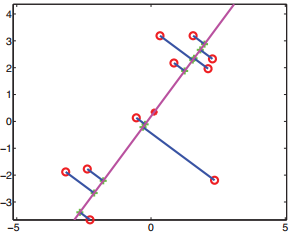
\includegraphics[scale=.60]{PCA-PPCA-a.png}} \\
\subfloat[]{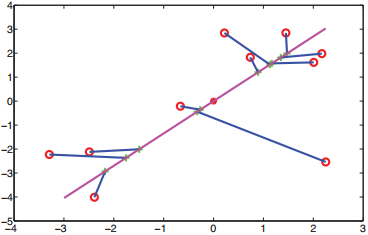
\includegraphics[scale=.60]{PCA-PPCA-b.png}}
\caption{An illustration of PCA and PPCA where $D=2$ and $L=1$. Circles are the original data points, crosses are the reconstructions. The red star is the data mean. (a) PCA. The points are orthogonally projected onto the line. (b) PPCA. The projection is no longer orthogonal: the reconstructions are shrunk towards the data mean (red star).}
\label{fig:PCA-PPCA} 
\end{figure}

The principal directions are the ones along which the data shows maximal variance. This means that PCA can be “misled” by directions in which the variance is high merely because of the measurement scale. It is therefore standard practice to standardize the data first, or equivalently, to work with correlation matrices instead of covariance matrices. 


\subsubsection{Proof *}
See Section 12.2.2 of MLAPP.


\subsection{Singular value decomposition (SVD)}
We have defined the solution to PCA in terms of eigenvectors of the covariance matrix. However, there is another way to obtain the solution, based on the \textbf{singular value decomposition}, or \textbf{SVD}. This basically generalizes the notion of eigenvectors from square matrices to any kind of matrix.

\begin{theorem}(\textbf{SVD}).
Any matrix can be decomposed as follows
\begin{equation}\label{eqn:SVD}
\underbrace{\vec{X}}_{N \times D}=\underbrace{\vec{U}}_{N \times N}\underbrace{\vec{\Sigma}}_{N \times D}\underbrace{\vec{V}^T}_{D \times D}
\end{equation}
where $\vec{U}$ is an $N \times N$ matrix whose columns are orthornormal(so $\vec{U}^T\vec{U}=\vec{I}$), $\vec{V}$ is $D \times D$ matrix whose rows and columns are orthonormal (so $\vec{V}^T\vec{V}=\vec{V}\vec{V}^T=\vec{I}_D$), and $\vec{\Sigma}$ is a $N \times D$ matrix containing the $r=\min(N,D)$ singular values $\sigma_i \geq 0$ on the main diagonal, with 0s filling the rest of the matrix.
\end{theorem}

This shows how to decompose the matrix $X$ into the product of three matrices: $\vec{V}$ describes an orthonormal basis in the domain, and $\vec{U}$ describes an orthonormal basis in the co-domain, and $\vec{\Sigma}$ describes how much the vectors in $\vec{V}$ are stretched to give the vectors in $\vec{U}$.

Since there are at most $D$ singular values (assuming $N>D$), the last $N−D$ columns of $\vec{U}$ are irrelevant, since they will be multiplied by 0. The \textbf{economy sized SVD}, or \textbf{thin SVD}, avoids computing these unnecessary elements. Let us denote this decomposition by $\hat{\vec{U}}\hat{\vec{\Sigma}}\hat{\vec{V}}^T$.If $N>D$, we have
\begin{equation}
\underbrace{\vec{X}}_{N \times D}=\underbrace{\hat{\vec{U}}}_{N \times D}\underbrace{\hat{\vec{\Sigma}}}_{D \times D}\underbrace{\hat{\vec{V}}^T}_{D \times D}
\end{equation}
as in Figure \ref{fig:SVD}(a). If $N<D$, we have
\begin{equation}
\underbrace{\vec{X}}_{N \times D}=\underbrace{\hat{\vec{U}}}_{N \times N}\underbrace{\hat{\vec{\Sigma}}}_{N \times N}\underbrace{\hat{\vec{V}}^T}_{N \times D}
\end{equation}
Computing the economy-sized SVD takes $O(ND\min(N,D))$ time (Golub and van Loan 1996, p254).

\begin{figure}[hbtp]
\centering
\subfloat[]{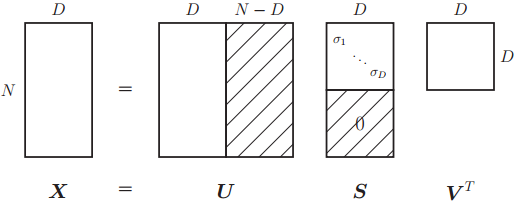
\includegraphics[scale=.50]{SVD-a.png}} \\
\subfloat[]{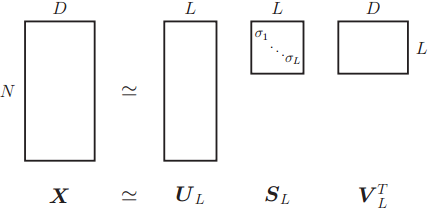
\includegraphics[scale=.50]{SVD-b.png}}
\caption{(a) SVD decomposition of non-square matrices $\vec{X}=\vec{U}\vec{\Sigma}\vec{V}^T$. The shaded parts of $\vec{\Sigma}$, and all the off-diagonal terms, are zero. The shaded entries in $\vec{U}$ and $\vec{\Sigma}$ are not computed in the economy-sized version, since they are not needed. (b) Truncated SVD approximation of rank $L$.}
\label{fig:SVD} 
\end{figure}

The connection between eigenvectors and singular vectors is the following:
\begin{align}
\vec{U}&=\mathrm{evec}(\vec{X}\vec{X}^T) \\
\vec{V}&=\mathrm{evec}(\vec{X}^T\vec{X}) \\
\vec{\Sigma}^2&=\mathrm{eval}(\vec{X}\vec{X}^T)=\mathrm{eval}(\vec{X}^T\vec{X})
\end{align}
For the proof please read Section 12.2.3 of MLAPP.

Since the eigenvectors are unaffected by linear scaling of a matrix, we see that the right singular vectors of $\vec{X}$ are equal to the eigenvectors of the empirical covariance $\hat{\vec{\Sigma}}$. Furthermore, the eigenvalues of $\hat{\vec{\Sigma}}$ are a scaled version of the squared singular values.

However, the connection between PCA and SVD goes deeper. From Equation \ref{eqn:SVD}, we can represent a rank $r$ matrix as follows:
\begin{equation*}
\vec{X}=\sigma_1\left(\begin{array}{c} | \\ \vec{u}_1 \\ | \end{array}\right)\left(\begin{array}{ccc} - & \vec{v}_1 & - \end{array}\right)+\cdots+\sigma_r\left(\begin{array}{c} | \\ \vec{u}_r \\ | \end{array}\right)\left(\begin{array}{ccc} - & \vec{v}_r^T & - \end{array}\right)
\end{equation*}
If the singular values die off quickly, we can produce a rank $L$ approximation to the matrix as follows:
\begin{align}
\vec{X} & \approx \sigma_1\left(\begin{array}{c} | \\ \vec{u}_1 \\ | \end{array}\right)\left(\begin{array}{ccc} - & \vec{v}_1 & - \end{array}\right)+\cdots+\sigma_r\left(\begin{array}{c} | \\ \vec{u}_L \\ | \end{array}\right)\left(\begin{array}{ccc} - & \vec{v}_L^T & - \end{array}\right) \nonumber \\
 & = \vec{U}_{:,1:L}\vec{\Sigma}_{1:L,1:L}\vec{V}_{:,1:L}^T
\end{align}
This is called a \textbf{truncated SVD} (see Figure \ref{fig:SVD}(b)).

One can show that the error in this approximation is given by
\begin{equation}
\lVert \vec{X}-\vec{X}_L \rVert_F \approx \sigma_L
\end{equation}
Furthermore, one can show that the SVD offers the best rank $L$ approximation to a matrix (best in the sense of minimizing the above Frobenius norm).

Let us connect this back to PCA. Let $\vec{X}=\vec{U}\vec{\Sigma}\vec{V}^T$ be a truncated SVD of $\vec{X}$. We know that $\hat{\vec{W}}=\vec{V}$, and that $\hat{\vec{Z}}=\vec{X}\hat{\vec{W}}$, so
\begin{equation}
\hat{\vec{Z}}=\vec{U}\vec{\Sigma}\vec{V}^T\vec{V}=\vec{U}\vec{\Sigma}
\end{equation}
Furthermore, the optimal reconstruction is given by $\hat{\vec{X}}=\vec{Z}\hat{\vec{W}}$,so we find
\begin{equation}
\hat{\vec{X}}=\vec{U}\vec{\Sigma}\vec{V}^T
\end{equation}
This is precisely the same as a truncated SVD approximation! This is another illustration of the fact that PCA is the best low rank approximation to the data.


\subsection{Probabilistic PCA}
\begin{theorem}((\textbf{Tipping and Bishop 1999})).
Consider a factor analysis model in which $\vec{\Psi}=\sigma^2\vec{I}$ and $\vec{W}$ is orthogonal. The observed data log likelihood is given by
\begin{align}
\log p(\vec{X}|\vec{W},\sigma^2\vec{I}) & =-\frac{N}{2}\ln|\vec{C}|-\frac{1}{2}\sum\limits_{i=1}^N \vec{x}_i^T\vec{C}^{-1}\vec{x}_i \nonumber \\
   & =-\frac{N}{2}\ln|\vec{C}|+\mathrm{tr}(\vec{C}^{-1}\vec{\Sigma})
\end{align}
where $\vec{C}=\vec{W}\vec{W}^T+\sigma^2\vec{I}$ and $\vec{\Sigma}=\frac{1}{N}\sum_{i=1}^N \vec{x}_i\vec{x}_i^T=\frac{1}{N}\vec{X}\vec{X}^T$. (We are assuming centred data, for notational simplicity.) The maxima of the log-likelihood are given by
\begin{equation}
\hat{\vec{W}}=\vec{V}(\vec{\Lambda}-\sigma^2\vec{I})^{\frac{1}{2}}\vec{R}
\end{equation}
where $\vec{R}$ is an arbitrary $L \times L$ orthogonal matrix, $\vec{V}$ is the $D \times L$ matrix whose columns are the first $L$ eigenvectors of $\vec{\Sigma}$, and $\vec{\Lambda}$ is the corresponding diagonal matrix of eigenvalues. Without loss of generality, we can set $\vec{R}=\vec{I}$. Furthermore, the MLE of the noise variance is given by
\begin{equation}
\hat{\sigma}^2=\frac{1}{D-L}\sum\limits_{j=L+1}^D \lambda_j
\end{equation}
which is the average variance associated with the discarded dimensions.
\end{theorem}

Thus, as $\sigma^2 \rightarrow 0$, we have $\hat{\vec{W}} \rightarrow \vec{V}$, as in classical PCA. What about $\hat{\vec{Z}}$? It is easy to see that the posterior over the latent factors is given by
\begin{align}
p(\vec{z}_i|\vec{x}_i,\hat{\vec{\theta}}) & = \mathcal{N}(\vec{z}_i|\hat{\vec{F}}^{-1}\hat{\vec{W}}^T\vec{x}_i,\sigma^2\hat{\vec{F}}^{-1}) \label{eqn:PPCA-posterior}\\
\hat{\vec{F}} & \triangleq \hat{\vec{W}}^T\hat{\vec{W}}+\sigma^2\vec{I}
\end{align}
(Do not confuse $\vec{F} = \vec{W}^T\vec{W}+\sigma^2\vec{I}$ with $\vec{C}=\vec{W}\vec{W}^T+\sigma^2\vec{I}$.) Hence, as $\sigma^2 \rightarrow 0$, we find $\hat{\vec{W}} \rightarrow \vec{V}$, $\hat{\vec{F}} \rightarrow \vec{I}$ and $\vec{z}_i \rightarrow \vec{V}^T\vec{x}_i$. Thus the posterior mean is obtained by an orthogonal projection of the data onto the column space of $\vec{V}$, as in classical PCA.

Note, however, that if $\sigma^2 \rightarrow 0$, the posterior mean is not an orthogonal projection, since it is shrunk somewhat towards the prior mean, as illustrated in Figure \ref{fig:PCA-PPCA}(b). This sounds like an undesirable property, but it means that the reconstructions will be closer to the overall data mean, $\hat{\vec{\mu}}=\bar{\vec{x}}$.


\subsection{EM algorithm for PCA}
\label{sec:EM-for-PCA}
Although the usual way to fit a PCA model uses eigenvector methods, or the SVD, we can also use EM, which will turn out to have some advantages that we discuss below. EM for PCA relies on the probabilistic formulation of PCA. However the algorithm continues to work in the zero noise limit, $\sigma^2=0$, as shown by (Roweis 1997).

Let $\tilde{\vec{Z}}$ be a $L \times N$ matrix storing the posterior means (low-dimensional representations) along its columns. Similarly, let $\tilde{\vec{X}}=\vec{X}^T$ store the original data along its columns. From Equation \ref{eqn:PPCA-posterior}, when $\sigma^2=0$, we have
\begin{equation}
\tilde{\vec{Z}}=(\vec{W}^T\vec{W})^{-1}\vec{W}^T\tilde{\vec{X}}
\end{equation}
This constitutes the E step. Notice that this is just an orthogonal projection of the data.

From Equation \ref{eqn:FA-EM-W}, the M step is given by
\begin{equation}
\hat{\vec{W}}=\left(\sum\limits_{i=1}^N \vec{x}_i\mathbb{E}[\vec{z}_i]^T\right)\left(\sum\limits_{i=1}^N \mathbb{E}[\vec{z}_i]\mathbb{E}[\vec{z}_i]^T\right)^{-1}
\end{equation}
where we exploited the fact that $\vec{\Sigma}=\mathrm{cov}[\vec{z}_i|\vec{x}_i,\vec{\theta}]=\vec{0}$ when $\sigma^2=0$.

(Tipping and Bishop 1999) showed that the only stable fixed point of the EM algorithm is the globally optimal solution. That is, the EM algorithm converges to a solution where $\vec{W}$ spans the same linear subspace as that defined by the first $L$ eigenvectors. However, if we want $\vec{W}$ to be orthogonal, and to contain the eigenvectors in descending order of eigenvalue, we have to orthogonalize the resulting matrix (which can be done quite cheaply). Alternatively, we can modify EM to give the principal basis directly (Ahn and Oh 2003).

This algorithm has a simple physical analogy in the case $D=2$ and $L=1$(Roweis 1997). Consider some points in $\mathbb{R}^2$ attached by springs to a rigid rod, whose orientation is defined by a vector $\vec{w}$. Let $\vec{z}_i$ be the location where the $i$'th spring attaches to the rod. See Figure 12.11 of MLAPP for an illustration.

Apart from this pleasing intuitive interpretation, EM for PCA has the following advantages over eigenvector methods:
\begin{itemize}
\item{EM can be faster. In particular, assuming $N,D \gg L$, the dominant cost of EM is the projection operation in the E step, so the overall time is $O(TLND)$, where $T$ is the number of iterations. This is much faster than the $O(\min(ND^2,DN^2))$ time required by straightforward eigenvector methods, although more sophisticated eigenvector methods, such as the Lanczos algorithm, have running times comparable to EM.}
\item{EM can be implemented in an online fashion, i.e., we can update our estimate of $\vec{W}$ as the data streams in.}
\item{EM can handle missing data in a simple way (see Section \ref{sec:Fitting-FA-models-with-missing-data}).}
\item{EM can be extended to handle mixtures of PPCA/ FA models.}
\item{EM can be modified to variational EM or to variational Bayes EM to fit more complex models.}
\end{itemize}


\section{Choosing the number of latent dimensions}
\label{sec:FA-Choosing-L}
In Section \ref{sec:Model-selection-for-LVM}, we discussed how to choose the number of components $K$ in a mixture model. In this section, we discuss how to choose the number of latent dimensions $L$ in a FA/PCA model.


\subsection{Model selection for FA/PPCA}
TODO

\subsection{Model selection for PCA}
TODO



\section{PCA for categorical data}
In this section, we consider extending the factor analysis model to the case where the observed data is categorical rather than real-valued. That is, the data has the form $y_{ij} \in \{1,...,C\}$, where $j=1:R$ is the number of observed response variables. We assume each $y_{ij}$ is generated from a latent variable $\vec{z}_i \in \mathbb{R}^L$, with a Gaussian prior, which is passed through the softmax function as follows:
\begin{align}
p(\vec{z}_i) & = \mathcal{N}(\vec{z}_i|\vec{0},\vec{I}) \\
p(\vec{y}_i|\vec{z}_i,\vec{\theta}) & = \prod\limits_{j=1}^R \mathrm{Cat}(y_{ir}|\mathcal{S}(\vec{W}_r^T\vec{z}_i+\vec{w}_{0r}))
\end{align}
where $\vec{W}_r \in \mathbb{R}^L$ is the factor loading matrix for response $j$, and $\vec{W}_{0r} \in \mathbb{R}^M$ is the offset term for response $r$, and $\vec{\theta}=(\vec{W}_r,\vec{W}_{0r})_{r=1}^R$. (We need an explicit offset term, since clamping one element of $\vec{z}_i$ to 1 can cause problems when computing the posterior covariance.) As in factor analysis, we have defined the prior mean to be $\vec{\mu}_0=\vec{0}$ and the prior covariance $\vec{V}_0=\vec{I}$, since we can capture non-zero mean by changing $\vec{w}_{0j}$ and non-identity covariance by changing $\vec{W}_r$. We will call this categorical PCA. See Chapter 27 TODO for a discussion of related models.

In (Khan et al. 2010), we show that this model outperforms finite mixture models on the task of imputing missing entries in design matrices consisting of real and categorical data. This is useful for analysing social science survey data, which often has missing data and variables of mixed type.


\section{PCA for paired and multi-view data}


\subsection{Supervised PCA (latent factor regression)}


\subsection{Discriminative supervised PCA}


\subsection{Canonical correlation analysis}


\section{Independent Component Analysis (ICA)}
\label{sec:ICA}
Let $\vec{x}_t \in \mathbb{R}^D$ be the observed signal at the sensors at “time” $t$, and $\vec{z}_t \in \mathbb{R}^L$ be the vector of source signals. We assume that
\begin{equation}
\vec{x}_t=\vec{W}\vec{z}_t+\vec{\epsilon}_t
\end{equation}
where $\vec{W}$ is an $D \times L$ matrix, and $\vec{\epsilon}_t \sim \mathcal{N}(\vec{0},\vec{\Psi})$. In this section, we treat each time point as an independent observation, i.e., we do not model temporal correlation (so we could replace the $t$ index with $i$, but we stick with t to be consistent with much of the ICA literature). The goal is to infer the source signals, $p(\vec{z}_t|\vec{x}_t,\vec{\theta})$. In this context, $\vec{W}$ is called the \textbf{mixing matrix}. If $L=D$ (number of sources = number of sensors), it will be a square matrix. Often we will assume the noise level, $|\vec{\Psi}|$, is zero, for simplicity.

So far, the model is identical to factor analysis. However, we will use a different prior for $p(\vec{z}_t)$. In PCA, we assume each source is independent, and has a Gaussian distribution. We will now relax this Gaussian assumption and let the source distributions be any \emph{non-Gaussian} distribution
\begin{equation}
p(\vec{z}_t) =\prod\limits_{j=1}^L p_j(z_{tj})
\end{equation}
Without loss of generality, we can constrain the variance of the source distributions to be \vec{1}, because any other variance can be modelled by scaling the rows of $\vec{W}$ appropriately. The resulting model is known as \textbf{independent component analysis} or \textbf{ICA}.

The reason the Gaussian distribution is disallowed as a source prior in ICA is that it does not permit unique recovery of the sources. This is because the PCA likelihood is invariant to any orthogonal transformation of the sources $\vec{z}_t$ and mixing matrix $\vec{W}$. PCA can recover the best linear subspace in which the signals lie, but cannot uniquely recover the signals themselves.

ICA requires that $\vec{W}$ is square and hence invertible. In the non-square case (e.g., where we have more sources than sensors), we cannot uniquely recover the true signal, but we can compute the posterior $p(\vec{z}_t|\vec{x}_t,\hat{\vec{W}})$, which represents our beliefs about the source. In both cases, we need to estimate Was well as the source distributions $p_j$. We discuss how to do this below.


\subsection{Maximum likelihood estimation}
In this section, we discuss ways to estimate square mixing matrices $\vec{W}$ for the noise-free ICA model. As usual, we will assume that the observations have been centered; hence we can also assume $\vec{z}$ is zero-mean. In addition, we assume the observations have been whitened, which can be done with PCA. 

If the data is centered and whitened, we have $\mathbb{E}[\vec{x}\vec{x}^T]=\vec{I}$. But in the noise free case, we also have
\begin{equation}
\mathrm{cov}[\vec{x}]=\mathbb{E}[\vec{x}\vec{x}^T]=\vec{W}\mathbb{E}[\vec{z}\vec{z}^T]\vec{W}^T
\end{equation}
Hence we see that $\vec{W}$ must be orthogonal. This reduces the number of parameters we have to estimate from $D^2$ to $D(D-1)/2$. It will also simplify the math and the algorithms.

Let $\vec{V}=\vec{W}^{-1}$; these are often called the recognition weights, as opposed to $\vec{W}$, which are the generative weights.

Since $\vec{x}=\vec{W}\vec{z}$, we have, from Equation \ref{eqn:Multivariate-transformation},
\begin{align}
p_x(\vec{W}\vec{z}_t) & =p_z(\vec{z}_t)|\mathrm{det}(\vec{W}^{-1})| \nonumber \\
   & = p_z(\vec{V}\vec{x}_t)|\mathrm{det}(\vec{V})|
\end{align}
Hence we can write the log-likelihood, assuming $T$ iid samples, as follows:
\begin{equation*}
\frac{1}{T} \log p(\mathcal{D}|\vec{V})=\log|\mathrm{det}(\vec{V})|+\frac{1}{T}\sum\limits_{j=1}^L \sum\limits_{t=1}^T \log p_j(\vec{v}_j^T\vec{x}_t)
\end{equation*}
where $\vec{v}_j$ is the $j$'th row of $\vec{V}$. Since we are constraining $\vec{V}$ to be orthogonal, the first term is a constant, so we can drop it. We can also replace the average over the data with an expectation operator to get the following objective
\begin{equation}
\mathrm{NLL}(\vec{V})=\sum\limits_{j=1}^L \mathbb{E}[G_j(\vec{z}_j)]
\end{equation}
where $\vec{z}_j=\vec{v}_j^T\vec{x}$ and $G_j(\vec{z}) \triangleq -\log p_j(\vec{z})$. We want to minimize this subject to the constraint that the rows of $\vec{V}$ are orthogonal. We also want them to be unit norm, since this ensures that the variance of the factors is unity (since, with whitened data, $\mathbb{E}[\vec{v}_j^T\vec{x}]=\lVert \vec{v}_j \rVert^2$, which is necessary to fix the scale of the weights. In otherwords, $\vec{V}$ should be an orthonormal matrix.

It is straightforward to derive a gradient descent algorithm to fit this model; however, it is rather slow. One can also derive a faster algorithm that follows the natural gradient; see e.g., (MacKay 2003, ch 34) for details. A popular alternative is to use an approximate Newton method, which we discuss in Section \ref{sec:FastICA}. Another approach is to use EM, which we discuss in Section \ref{sec:ICA-EM}.


\subsection{The FastICA algorithm}
\label{sec:FastICA}


\subsection{Using EM}
\label{sec:ICA-EM}


\subsection{Other estimation principles *}

